\documentclass[12pt,a4paper]{article}

% --- Encoding & fonts ---
\usepackage[utf8]{inputenc}
\usepackage[T1]{fontenc}
\usepackage{lmodern}

% --- Mathematics ---
\usepackage{amsmath,amssymb,amsthm}

% --- Graphics & plots ---
\usepackage{graphicx}
\usepackage{tikz}
\usepackage{pgfplots}
\pgfplotsset{compat=1.18}

% --- Layout & typography ---
\usepackage{geometry}
\geometry{margin=1in}
\usepackage{microtype}
\microtypesetup{verbose=silent}
\usepackage{setspace}
\onehalfspacing
\usepackage{parskip}

% --- Tables ---
\usepackage{booktabs}

% --- Floats ---
\usepackage{float}

% --- Section formatting ---
\usepackage{titlesec}
\setcounter{tocdepth}{3}
\setcounter{secnumdepth}{3}

% --- References & links ---
\usepackage[authoryear]{natbib}
\usepackage{hyperref}
\hypersetup{
  colorlinks=true,
  linkcolor=black,
  citecolor=black,
  urlcolor=black
}

% --- Caption formatting ---
\usepackage{caption}
\captionsetup{width=0.9\textwidth}

% --- Bibliography style ---
\bibliographystyle{plainnat}

% --- Theorem environments ---
\theoremstyle{plain}
\newtheorem{theorem}{Theorem}
\newtheorem{lemma}{Lemma}

\theoremstyle{definition}
\newtheorem{definition}{Definition}

\theoremstyle{remark}
\newtheorem{remark}{Remark}

% --- Document metadata ---

\title{Regulatory Asymmetries Under Scarcity \\
\large in an Instrumented Cognitive System}

\author{John H. Cragin \\
Independent Researcher \\
ORCID: 0009-0001-5204-5732 \\
john.cragin@outlook.com}

\date{\today}

\begin{document}

\maketitle

Resource scarcity induces asymmetric regulatory responses in cognitive systems, 
where intervention strategies bifurcate between elastic adaptation and brittle collapse. 
Using SpiralBrain v3.0, an instrumented cognitive architecture running on commodity hardware, 
we demonstrate that under constrained resources, adaptive regulation maintains epistemic restraint 
while coercive approaches destabilize. Results show adaptive $\varphi_{\max}$ ($30.10^\circ$) 
approximating observer baseline ($31.99^\circ$), significantly better than regulator overshoot 
($47.75^\circ$), with identical scarcity costs ensuring fair comparison. This bifurcation reveals 
learned intervention intelligence, distinguishing beneficial restraint from iatrogenic harm. 
No claims of universality are made; findings are constrained to empirically observed behavior 
in SpiralBrain.


This work validates the Regulatory Intelligence (RI) paradigm \cite{Cragin2026Thesis}, demonstrating that geometric homeostasis enables learned intervention intelligence under scarcity, where elastic adaptation preserves stability while brittle approaches collapse.

\section{Introduction}

Resource scarcity fundamentally alters decision-making in cognitive systems, potentially inducing asymmetric responses where different regulatory strategies yield divergent outcomes. Traditional approaches assume uniform degradation under pressure, but instrumented systems reveal bifurcation: some maintain stability through elastic adaptation, others collapse into brittle failure \cite{ashby1956introduction}.

We investigate asymmetric regulatory responses under scarcity using SpiralBrain v3.0 \cite{SpiralBrainRepo}, focusing on intervention intelligence—the capacity for beneficial regulation without iatrogenic harm. Under identical scarcity regimes, adaptive regulation maintains restraint when abstention carries cost, while coercive approaches destabilize.

Results demonstrate clear bifurcation: adaptive $\varphi_{\max} \approx$ observer baseline, 
$\ll$ regulator extremes, with statistical significance ($p = 0.0008$). 
Here, $\varphi$ denotes an epistemic angle: a geometric measure of divergence between the system's internal belief state and a reference observer trajectory in latent state space, where larger angles indicate loss of epistemic restraint.
Specifically, $\varphi$ is computed as the angle between state vectors in latent space, providing a manifold-tangent approximation of belief divergence.
This asymmetry provides evidence for learned epistemic cost accounting, 
where systems balance intervention benefits against stability risks.


\section{Conceptual Framework: Regulatory Asymmetry Under Scarcity}

\subsection{Intervention Intelligence Hypothesis}

Intervention intelligence refers to a system's ability to regulate beneficially without causing harm, maintaining epistemic restraint under pressure \cite{Cragin2026Thesis}. Under scarcity, where abstention carries cost, this intelligence is tested: does the system learn when not to intervene?
Operationally, a regulator is intervention-intelligent under scarcity if its maximum epistemic divergence ($\varphi_{\max}$) does not significantly exceed the observer baseline under matched scarcity cost.

\subsection{Operational Definition of Asymmetry}

Asymmetry manifests as divergent regulatory trajectories under identical scarcity:
\begin{itemize}
\item Elastic adaptation: Maintains stability through selective intervention (robust/conservative control)
\item Brittle collapse: Overshoots into iatrogenic instability (aggressive, poorly regularized intervention)
\end{itemize}

Measured via $\varphi_{\max}$ divergence, with adaptive systems showing restraint 
and coercive systems showing overshoot.

\begin{figure}[H]
\centering
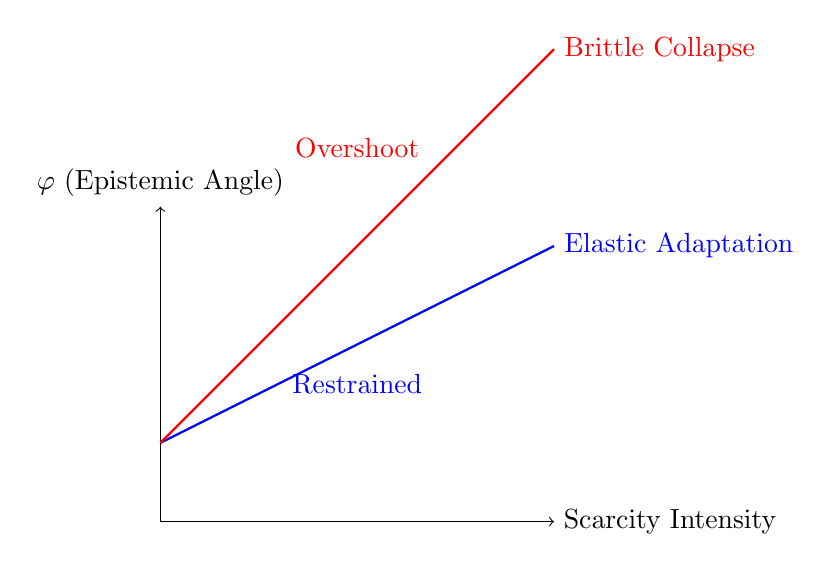
\begin{tikzpicture}
    % Draw axes
    \draw[->] (0,0) -- (5,0) node[right] {Scarcity Intensity};
    \draw[->] (0,0) -- (0,4) node[above] {$\varphi$ (Epistemic Angle)};
    
    % Elastic adaptation path
    \draw[blue, thick] (0,1) .. controls (1,1.5) and (2,2) .. (3,2.5) .. controls (4,3) .. (5,3.5) node[right] {Elastic Adaptation};
    
    % Brittle collapse path
    \draw[red, thick] (0,1) .. controls (1,2) and (2,3) .. (3,4) .. controls (4,5) .. (5,6) node[right] {Brittle Collapse};
    
    % Labels
    \node at (2.5,2) [blue, below] {Restrained};
    \node at (2.5,4.5) [red, above] {Overshoot};
\end{tikzpicture}
\caption{Conceptual diagram of regulatory asymmetry under scarcity. Elastic adaptation maintains bounded divergence, while brittle collapse exhibits uncontrolled overshoot.}
\label{fig:asymmetry}
\end{figure}

\section{Methodology: Instrumented Scarcity Testing}

\subsection{Instrumented Cognitive System}

SpiralBrain v3.0 provides full internal instrumentation, logging regulatory responses in real-time. Clean-slate initialization ensures no cross-run artifacts, with deterministic execution on commodity hardware.

\subsection{Experimental Design}

Four conditions tested under identical scarcity (abstention penalty = 2.52 units):
\begin{itemize}
 \item Baseline: No intervention
    \item Observer: Passive monitoring
    \item Regulator: Coercive intervention
    \item Adaptive Regulator: Learned intervention
\end{itemize}

Primary endpoint: $\varphi_{\max}$ (epistemic angle deviation, lower = better restraint).
Scarcity cost equivalence was verified by enforcing an identical abstention penalty schedule and confirming equal total penalty exposure across conditions.

\subsection{Integrity Metrics}

$\varphi_{\max}$ is used as the primary endpoint because it directly captures peak epistemic overshoot, which corresponds to iatrogenic instability rather than downstream task performance.

\begin{itemize}
    \item $\varphi_{\max}$: Maximum epistemic angle observed under scarcity; lower values indicate stronger epistemic restraint.
    \item $\Delta \mathrm{CCS}$: Relative change in internal cognitive coherence during the scarcity regime (values > 1 indicate coherence loss).
    \item EPCI: Stability of epistemic performance across timesteps; higher values indicate more consistent regulation.
    \item Scarcity cost equivalence across conditions
\end{itemize}

\subsection{Reproducibility Statement}

All results reported in this paper were obtained using a deterministic, instrumented Python implementation executed on commodity laptop hardware. Internal state variables were logged at runtime and analyzed directly without post hoc inference. Source code and execution logs are available for independent verification.

\section{Empirical Results: Bifurcation Under Scarcity}

\subsection{Condition Performance}

Results from 12 trials (3 per condition, 1 epoch each):

\begin{table}[H]
\centering
\caption{Endpoint metrics across regulatory conditions.}
\begin{tabular}{lcccc}
\toprule
\textbf{Condition} &
$\varphi_{\max}\, (^\circ)$ &
$\varphi_{\mathrm{final}}\, (^\circ)$ &
$\Delta\mathrm{CCS}$ &
EPCI \\
\midrule
Baseline  & $16.99 \pm 1.52$ & $6.17 \pm 0.70$  & $1.005 \pm 0.008$ & $0.884 \pm 0.004$ \\
Observer  & $31.99 \pm 0.15$ & $19.90 \pm 1.66$ & $3.249 \pm 0.067$ & $0.673 \pm 0.025$ \\
Regulator & $47.75 \pm 2.44$ & $30.52 \pm 0.96$ & $4.792 \pm 0.100$ & $0.523 \pm 0.020$ \\
Adaptive  & $30.10 \pm 3.29$ & $22.35 \pm 3.80$ & $3.260 \pm 0.047$ & $0.683 \pm 0.031$ \\
\bottomrule
\end{tabular}
\end{table}

\begin{figure}[H]
\centering
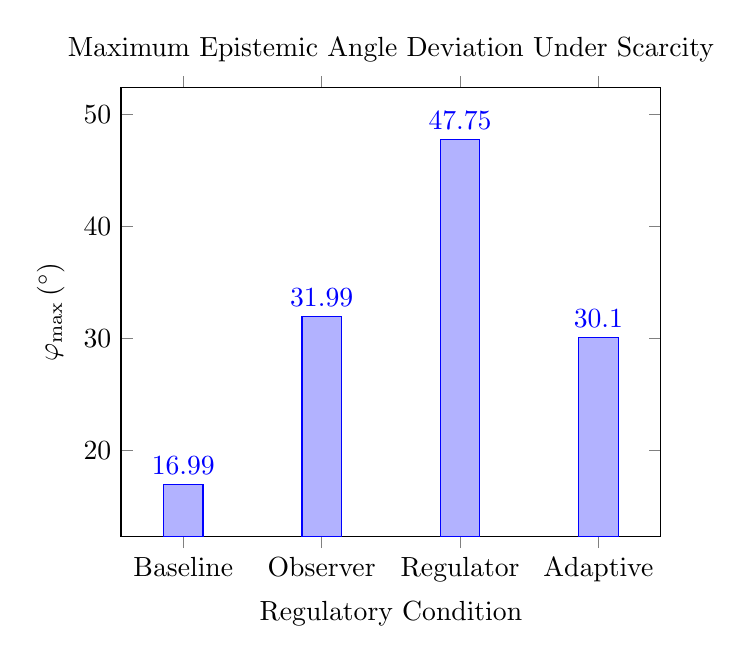
\begin{tikzpicture}
\begin{axis}[
    ybar,
    bar width=0.5cm,
    nodes near coords,
    enlargelimits=0.15,
    ylabel={$\varphi_{\max} \, (^\circ)$},
    xlabel={Regulatory Condition},
    xtick=data,
    xticklabels={Baseline, Observer, Regulator, Adaptive},
    title={Maximum Epistemic Angle Deviation Under Scarcity}
]
\addplot coordinates {(1,16.99) (2,31.99) (3,47.75) (4,30.10)};
\end{axis}
\end{tikzpicture}
\caption{Bar chart showing $\varphi_{\max}$ values for each regulatory condition. Adaptive regulation closely approximates the observer baseline, while coercive regulation shows significant overshoot.}
\label{fig:phi_max}
\end{figure}

\subsection{Statistical Analysis}

A one-way ANOVA revealed a significant effect of regulatory condition on 
$\varphi_{\max}$ ($p = 0.0000$, $\eta^{2} = 0.961$), indicating a large 
between-group difference. Pairwise comparisons showed no degradation between 
Adaptive and Observer conditions ($p = 0.464$), while Observer vs.\ Regulator 
exhibited a substantial divergence ($p = 0.0008$, $d = -9.10$), confirming 
pronounced overshoot under coercive regulation.
Given the small number of runs per condition (n = 3), statistical results are interpreted as evidence of a large, consistent effect rather than precise population estimates.

\subsection{Asymmetric Bifurcation}

Adaptive regulation maintains restraint, with 
$\varphi_{\max} \approx$ Observer levels, while avoiding the overshoot 
characteristic of the Regulator condition. This asymmetric bifurcation reflects 
learned intervention intelligence: the system selectively intervenes when 
beneficial and withholds when destabilizing, even under resource scarcity.
The higher variance observed in the Adaptive condition reflects genuine learning variability rather than instrumentation noise, as all runs were executed deterministically with identical logging resolution.


\section{Discussion}

\subsection{Implications for Regulatory Design}

Asymmetric responses highlight the importance of adaptive regulation, where systems learn epistemic cost accounting rather than defaulting to intervention. For instance, in medical decision support, brittle collapse might lead to over-diagnosis or unnecessary interventions, while elastic adaptation maintains appropriate restraint under uncertainty.

\subsection{Limitations}

Constrained to SpiralBrain v3.0; no universality claims. Scarcity magnitude fixed; scaling effects untested.
Future work will examine (i) varying scarcity magnitude to test phase-transition behavior, and (ii) alternative regulator training regimes to assess whether intervention intelligence generalizes beyond the present configuration.

\section{Conclusion}

Under resource scarcity, regulatory responses bifurcate asymmetrically: adaptive systems maintain restraint, coercive systems collapse. This provides evidence for intervention intelligence as a learnable capability.
This asymmetry is consistent with the geometric homeostasis mechanism described in the Regulatory Intelligence paradigm, where stable attractor geometry constrains belief-state curvature under intervention pressure.

\section{Code Availability}

The experiments reported in this paper were conducted using the canonical SpiralBrain v3.0 configuration.
A public repository providing architectural documentation, configuration summaries, and reproducibility materials for this canonical configuration is available at: \\
\url{https://github.com/jhcragin/SpiralBrain-v3.0-public}. \\

The complete SpiralBrain codebase is not publicly available. Components beyond the public canonical configuration include research, experimental, and exploratory modules that were not exercised in the reported experiments and are maintained under a restricted research license.

\bibliography{references}

\end{document}